% !TEX encoding = UTF-8 Unicode
\documentclass[a4paper]{article}

\usepackage{color}
\usepackage{url}
\usepackage[T2A]{fontenc} % enable Cyrillic fonts
\usepackage[utf8]{inputenc} % make weird characters work
\usepackage{graphicx}

\usepackage[english,serbian]{babel}
%\usepackage[english,serbianc]{babel} %ukljuciti babel sa ovim opcijama, umesto gornjim, ukoliko se koristi cirilica

\usepackage[unicode]{hyperref}
\hypersetup{colorlinks,citecolor=blue,filecolor=green,linkcolor=blue,urlcolor=blue}

\usepackage{listings}

%\newtheorem{primer}{Пример}[section] %ćirilični primer
\newtheorem{primer}{Primer}[section]

\definecolor{mygreen}{rgb}{0,0.6,0}
\definecolor{mygray}{rgb}{0.5,0.5,0.5}
\definecolor{mymauve}{rgb}{0.58,0,0.82}

\lstset{ 
  backgroundcolor=\color{white},   % choose the background color; you must add \usepackage{color} or \usepackage{xcolor}; should come as last argument
  basicstyle=\scriptsize\ttfamily,        % the size of the fonts that are used for the code
  breakatwhitespace=false,         % sets if automatic breaks should only happen at whitespace
  breaklines=true,                 % sets automatic line breaking
  captionpos=b,                    % sets the caption-position to bottom
  commentstyle=\color{mygreen},    % comment style
  deletekeywords={...},            % if you want to delete keywords from the given language
  escapeinside={\%*}{*)},          % if you want to add LaTeX within your code
  extendedchars=true,              % lets you use non-ASCII characters; for 8-bits encodings only, does not work with UTF-8
  firstnumber=1000,                % start line enumeration with line 1000
  frame=single,	                   % adds a frame around the code
  keepspaces=true,                 % keeps spaces in text, useful for keeping indentation of code (possibly needs columns=flexible)
  keywordstyle=\color{blue},       % keyword style
  language=Python,                 % the language of the code
  morekeywords={*,...},            % if you want to add more keywords to the set
  numbers=left,                    % where to put the line-numbers; possible values are (none, left, right)
  numbersep=5pt,                   % how far the line-numbers are from the code
  numberstyle=\tiny\color{mygray}, % the style that is used for the line-numbers
  rulecolor=\color{black},         % if not set, the frame-color may be changed on line-breaks within not-black text (e.g. comments (green here))
  showspaces=false,                % show spaces everywhere adding particular underscores; it overrides 'showstringspaces'
  showstringspaces=false,          % underline spaces within strings only
  showtabs=false,                  % show tabs within strings adding particular underscores
  stepnumber=2,                    % the step between two line-numbers. If it's 1, each line will be numbered
  stringstyle=\color{mymauve},     % string literal style
  tabsize=2,	                   % sets default tabsize to 2 spaces
  title=\lstname                   % show the filename of files included with \lstinputlisting; also try caption instead of title
}

\begin{document}

\title{Razvoj LSTM neuronske mreže i primena nad problemom sekvencijalnog učenja\\ \small{Seminarski rad u okviru kursa\\Računarska inteligencija\\ Matematički fakultet}}

\author{Milena Kurtić, Nevena Soldat\\ mimikurtic67@gmail.com, nevenasoldat@gmail.com}

%\date{14.~april 2015.}

\maketitle

\abstract{
U okviru ovog rada predstavljen je primer implementacije LSTM neuronske mreže u programskom jeziku Python, uz korišćenje biblioteka za rad kao što su pandas, numpy, keras i druge. Prvi deo rada opisuje teorijsku osnovu iza ovih mreža. Zatim je opisana primena na problem generisanja teksta. 
Videćemo koje su njene prednosti, kao i ograničenja. Pokazana je razlika u ponašanju modela sa različitim konfiguracijama. }

\tableofcontents

\newpage

\section{Uvod}
\label{sec:uvod}

Neuronske mreže (eng. neural networks) predstavljaju najpopularniju i jednu od najprimenjenijih metoda mašinskog učenja. Njihove primene su mnogobrojne i pomeraju domete veštačke inteligencije, računarstva i primenjene matematike. Postoji više vrsta neuronskih mreža: potpuno povezane, konvolutivne, rekurentne, grafovske neuronske mreže. U vrstu rekurentnih spada i LSTM neuronska mreza.

Osnovna ideja veštačke neuronske mreže je simulacija velike količine gusto napakovanih, međusobno  povezanih nervnih  ćelija u okviru računara, tako da je omogućeno učenje pojmova, prepoznavanje šablona i donošenje odluka na način koji je sličan čovekovom. Suštinski, veštačke neuronske mreže su softverske simulacije, napravljene programirajući obične računare koji rade u uobičajenom režimu sa svojim tranzistorima i serijski povezanim logičkim  kolima, tako da se ponašaju kao da su napravljene od milijardu međusobno povezanih ćelija mozga koje rade paralelno. 

\subsection{Opis rada}

U ovom radu je implementirana rekurentna neuronska mreža koja automatski generiše određeni tekst. Podaci koje koristimo predstavljaju kratke opise filmova. Cilj nam je da za određenu sekvencu reči uspemo da pretpostavimo koja će biti sledeća. Korišćena je posebna verzija rekurentne mreže koja ume da pamti duge sekvence - kratka dugoročna memorija (eng. Long Short Term Memory - LSTM). 

Mnogi radovi bave se automatskim generisanjem teksta. Rad koji je sličan našem opisuje automatsko generisanje kratkih priča na nivou generisanja pojedinačnih reči  \cite{pawade2018story}. Automatsko generisanje teksta može biti implementirano i na nivou karaktera, što je opisano u radu \cite{sutskever2011generating}.

LSTM mreže koriste se za razne probleme nad sekvencijalnim podacima. Tako imamo radove koji se bave automatskim generisanjem reči pesama \cite{potash2015ghostwriter}, ili čak automatskim komponovanjem muzike \cite{choi2016text}.

\section{Rekurentne neuronske mreže}
Rekurentne neuronske mreže (eng. Recurrent Neural Networks - RNN) predstavljaju arhitekturu mreža specijalizovanu za obradu sekvencijalnih podataka, poput rečenica prirodnog jezika i vremenskih serija. Sekvence nameću važnost redosleda zapažanja podataka, kako prilikom treniranja modela, tako i prilikom predviđanja. Mreže su konstruisane sa idejom da se modeluje zavisnost među instancama. Elementi ulazne sekvence se obrađuju u koracima, mreža ima skriveno stanje koje akumulira informaciju o elementiam sekvence obrađenim u prethodnim koracima, a parametri određuju na koji način se to stanje menja iz koraka u korak na osnovu prethodnog stanja i tekućih ulaza i kako se generiše izlaz u zavisnosti od tekućeg stanja.

"Learning of sequential data continues to be a fundamental task and a challenge in
pattern recognition and machine learning. Applications involving sequential data
may require prediction of new events, generation of new sequences, or decision
making such as classification of sequences or sub-sequences."

     — On Prediction Using Variable Order Markov Models, 2004.

\subsection{Arhitektura RNN}

Rekurentne neuronske mreže sadrže petlje koje obezbeđuju čuvanje informacija \cite{understandingLSTM}.

\begin{figure}[htp]
    \centering
    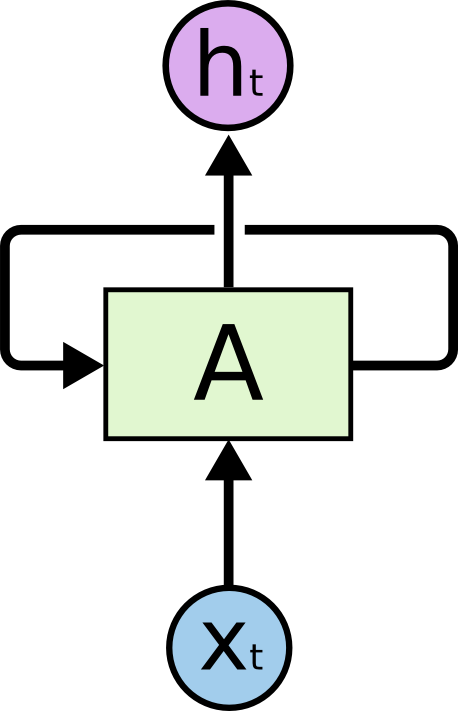
\includegraphics[scale=0.4]{RNN-rolled.png}
    \caption{Prikaz RNN mreže}
    \label{fig:rnn}
\end{figure}

Na slici \ref{fig:rnn} prikazan je jedan deo neuronske mreže, A, čiji je ulaz $x_t$, a izlaz $h_t$. Petlja omogućava da se informacije prosleđuju iz jednog koraka u mreži u drugi. Biće jednostavnije ako ih zamislimo na sledeći način:

\begin{figure}[htp]
    \centering
    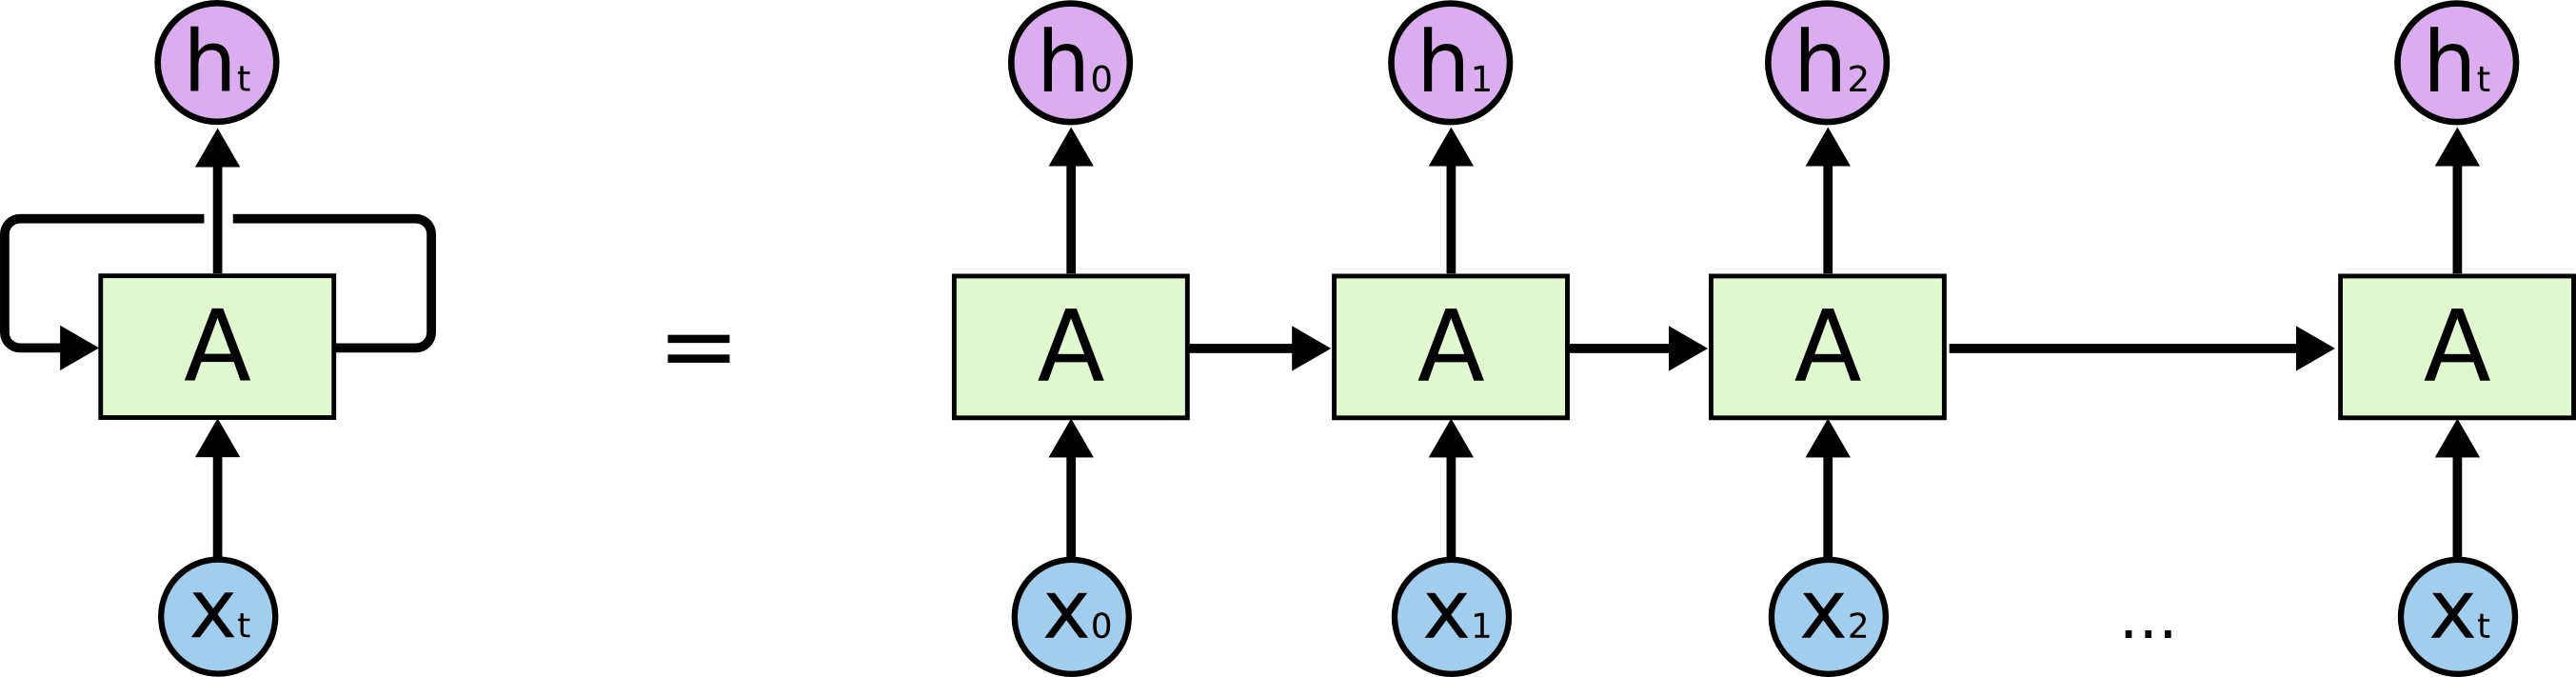
\includegraphics[scale=0.4]{RNN-unrolled.png}
    \caption{Prikaz RNN mreže u obliku lanca}
    \label{fig:rnn2}
\end{figure}

Rekurentna mreža predstavlja veći broj istih mreža, koje prenose poruke narednom delu u lancu, što je prikazano na slici \ref{fig:rnn2}. 

\subsection{Problemi sa RNN}
Postoje dva osnovna problema rekurentnih neuronskih mreža u njihovoj osnovnoj formi. Prvi se tiče problema nestajućih i eksplodirajućih gradijenata. Naime, graf izračunavanja rekurentne neuronske mreže je tipično vrlo dubok zbog velike dužine sekvence. Usled toga, prilikom izračunavanja gradijenta propagacijom u prošlost, dolazi do velikog broja množenja koja neretko čine da koordinate gradijenta ili eksplodiraju ili nestanu.

Drugi problem se odnosi na dugoročno čuvanje informacije i modelovanje dugoročnih zavisnosti u podacima. Kako se skriveno stanje u svakom koraku dobija linearnom kombinacijom prethodnog stanja i ulaza, doprinos starijih ulaza se brzo gubi pod uticajem novih. Dugoročno čuvanje relevantnih informacija nije moguće.

Oba ova problema se prevazilaze upotrebom duge kratkoročne memorije (eng. long short term memory), skraćeno LSTM, što je složena jedinica mreže sa specifičnom strukturom koja omogućava kontrolu čitanja i upisa u jedinicu. Upravo ova jedinica dovela je do ključnih uspeha rekurentnih neuronskih mreža i predstavlja standardni izbor prilikom formulisanja modela rekurentne mreže. \cite{matf}


\subsection{LSTM neuronske mreže}

LSTM neuronske mreže su specijalizovane za prevazilaženje problema kratkotrajne memorije. Pamćenje dugih sekvenci je praktično njihovo podrazumevano ponašanje, a ne nešto sa čime se muče. Kao što je već prikazano, sve rekurentne mreže imaju lančanu formu, sastavljenu od modula mreže koji se ponavljaju. Kod LSTM mreža, struktura ovih modula je malo drugačija. Umesto jednog sloja mreže, imamo četiri koja su povezana na veoma poseban način (Slika \ref{fig:lstm3}).

\begin{figure}[htp]
    \centering
    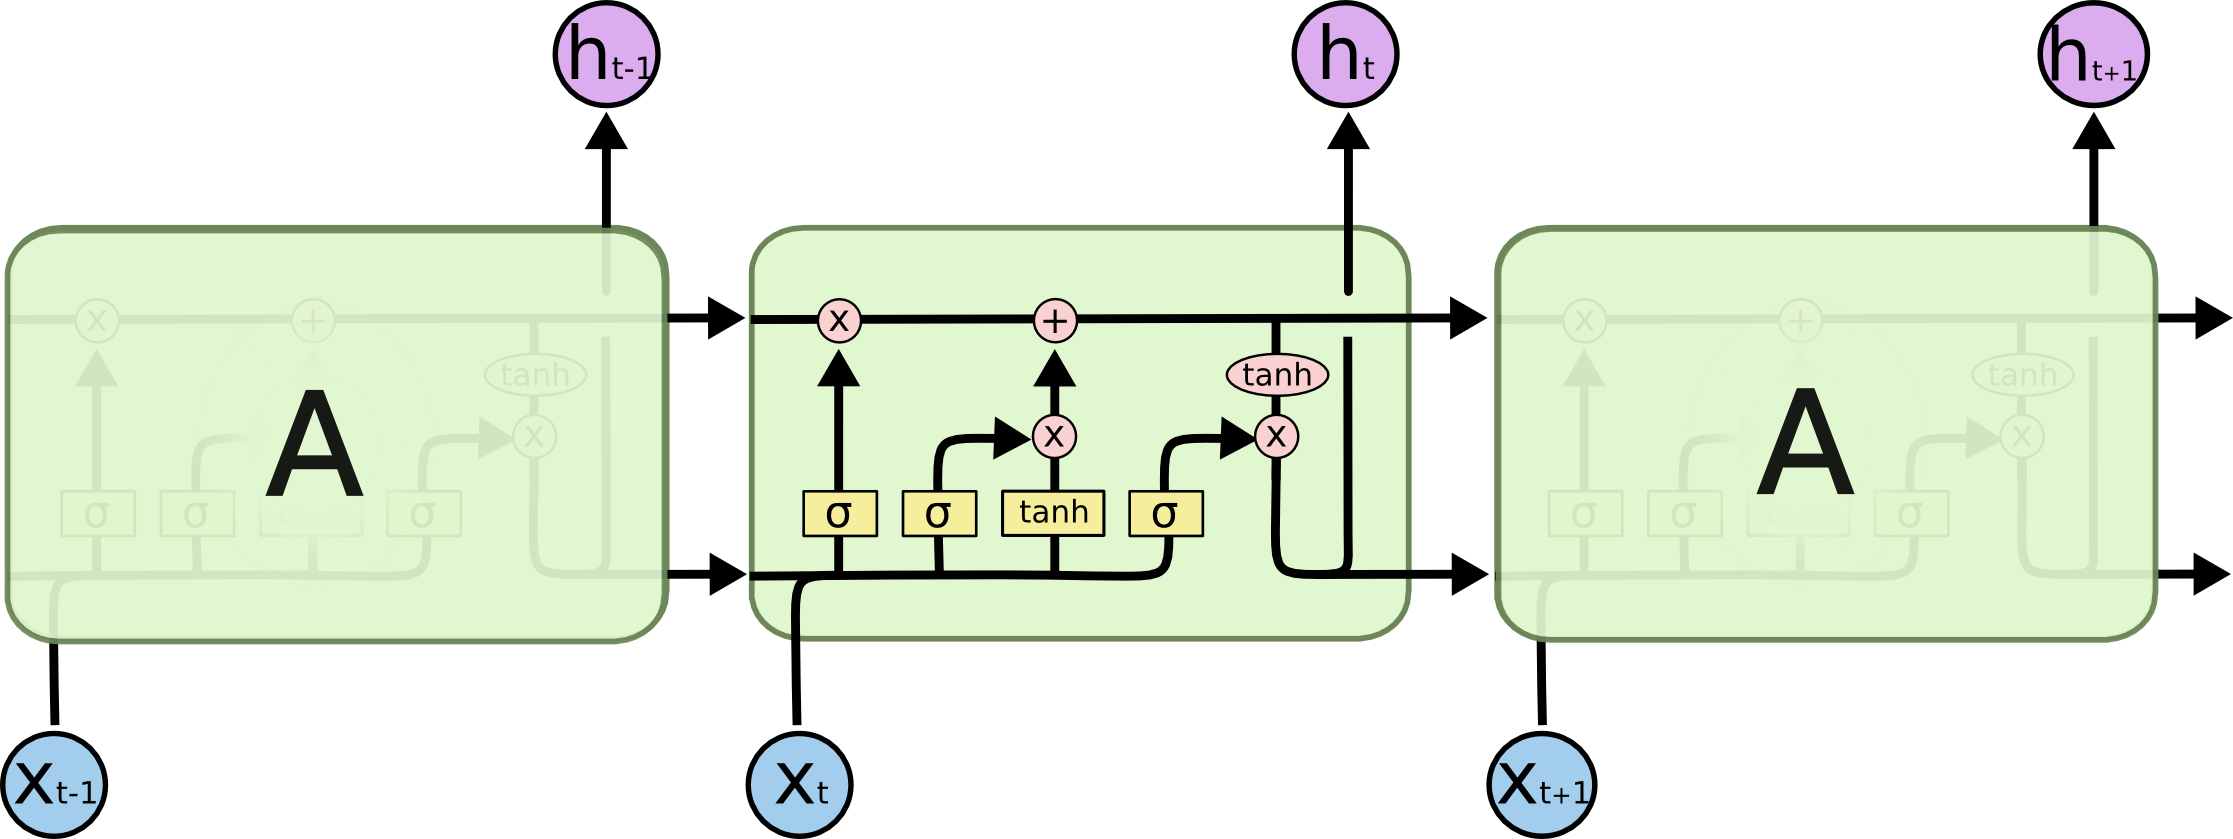
\includegraphics[scale=0.3]{LSTM3-chain.png}
    \caption{Prikaz lanca LSTM mreže}
    \label{fig:lstm3}
\end{figure}

Na slici iznad, svaka linija prenosi vektor podataka, od izlaza iz prethodnog čvora, do ulaza u naredni. Roze krugovi predstavljaju operacije, poput sabiranja vektora, dok žuti pravougaonici predstavljaju slojeve mreže. Linije koje se spajaju obeležavaju spajanje informacija, dok linije koje se razdvajaju predstavljaju sadržaj koji se kopira, gde kopije idu na različita mesta (Slika \ref{fig:lstm4}).

\begin{figure}[htp]
    \centering
    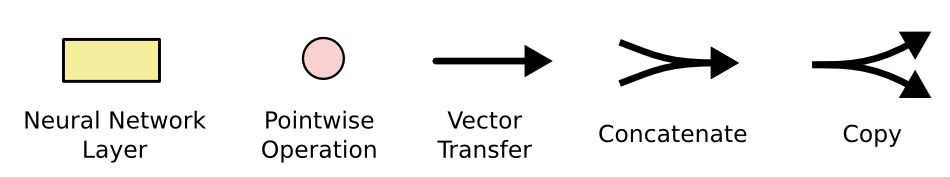
\includegraphics[scale=0.3]{LSTM2-notation.png}
    \caption{Notacija}
    \label{fig:lstm4}
\end{figure}

Osnovna ideja LSTM-a je postojanje takozvane ćelije koja čuva skriveno stanje, uz kontrolu pisanja, čitanja i zaboravljanja. Na slici \ref{fig:lstm5} je to horizontalna linija na vrhu dijagrama.

\begin{figure}[htp]
    \centering
    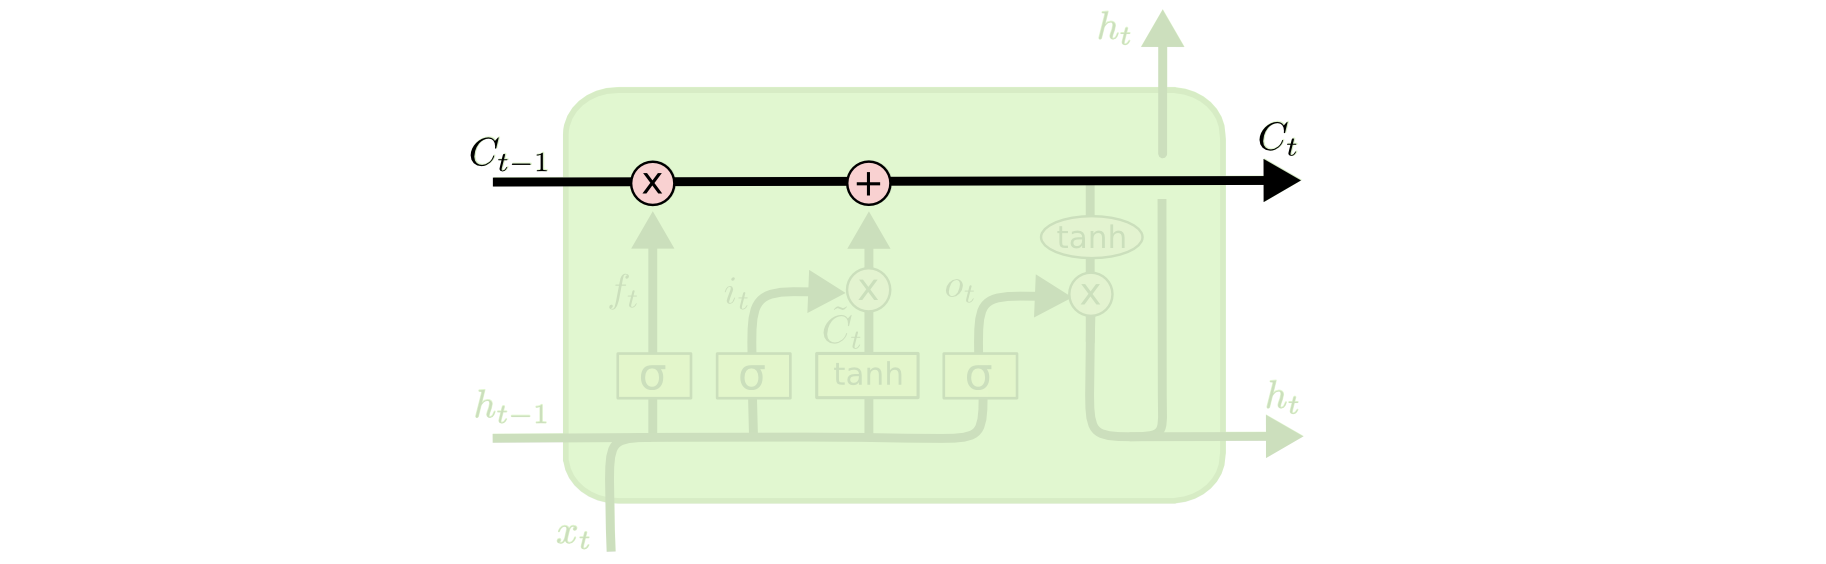
\includegraphics[scale=0.4]{LSTM3-C-line.png}
    \caption{Ćelija LSTM mreže}
    \label{fig:lstm5}
\end{figure}


Stanje ćelije prolazi kroz ceo lanac, uz male linearne interakcije. Informacije se veoma lako prenose nepromenjene. LSTM može da doda ili ukloni informacije iz stanja ćelije, pomoću struktura koje se nazivaju kapije. Kapije odlučuju koje informacije i u kojoj količini će biti očuvane. 

Prvi korak u našoj LSTM mreži je odabir informacija koje će biti obrisane iz stanja ćelije. Kapija koja kontroliše ovu operaciju naziva se ,,kapija zaboravljanja``. Ovaj sloj koristi sigmoidnu aktivacionu funkciju, čiji je izlaz interval brojeva između 0 i 1. Vrednost 1 znači da se potpuno zadržava sadržaj, a 0 da se potpuno briše (Slika \ref{fig:lstm6}).


\begin{figure}[htp]
    \centering
    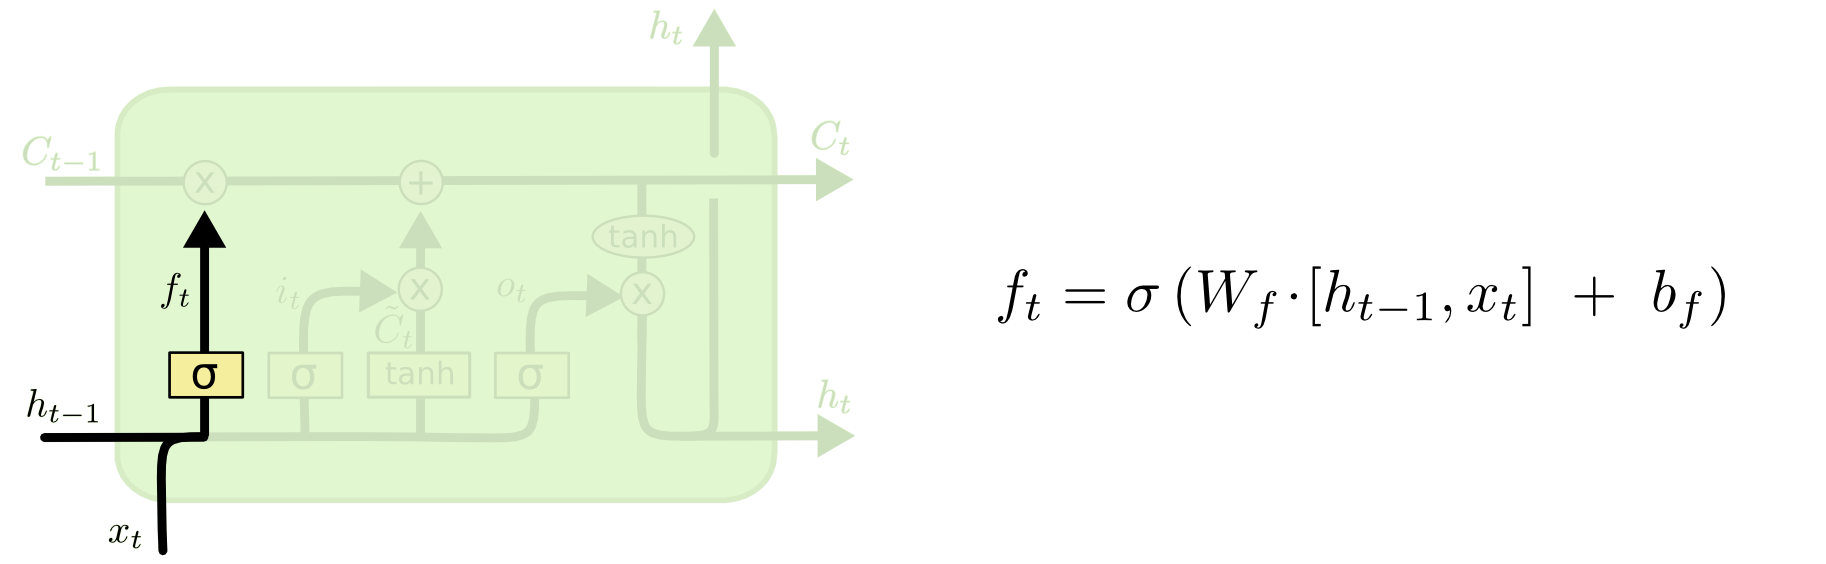
\includegraphics[scale=0.4]{LSTM3-focus-f.png}
    \caption{Kapija zaboravljanja}
    \label{fig:lstm6}
\end{figure}

Sledeći korak predstavlja odlučivanje o tome koje nove informacije ćemo dodati u stanje ćelije. Sastoji se iz dva dela. Prvo, sloj koji predstavlja ,,ulaznu kapiju`` odlučuje koje će vrednosti ažurirati. Zatim naredni sloj, čija je aktivaciona funkcija tangens hiperbolički, pravi vektor novih vrednosti ($\tilde{C}_t$), koje se mogu dodati u stanje ćelije. U sledećem koraku kombinujemo ova dva dela i pravimo novo stanje ćelije (Slika \ref{fig:lstm7}).

\begin{figure}[htp]
    \centering
    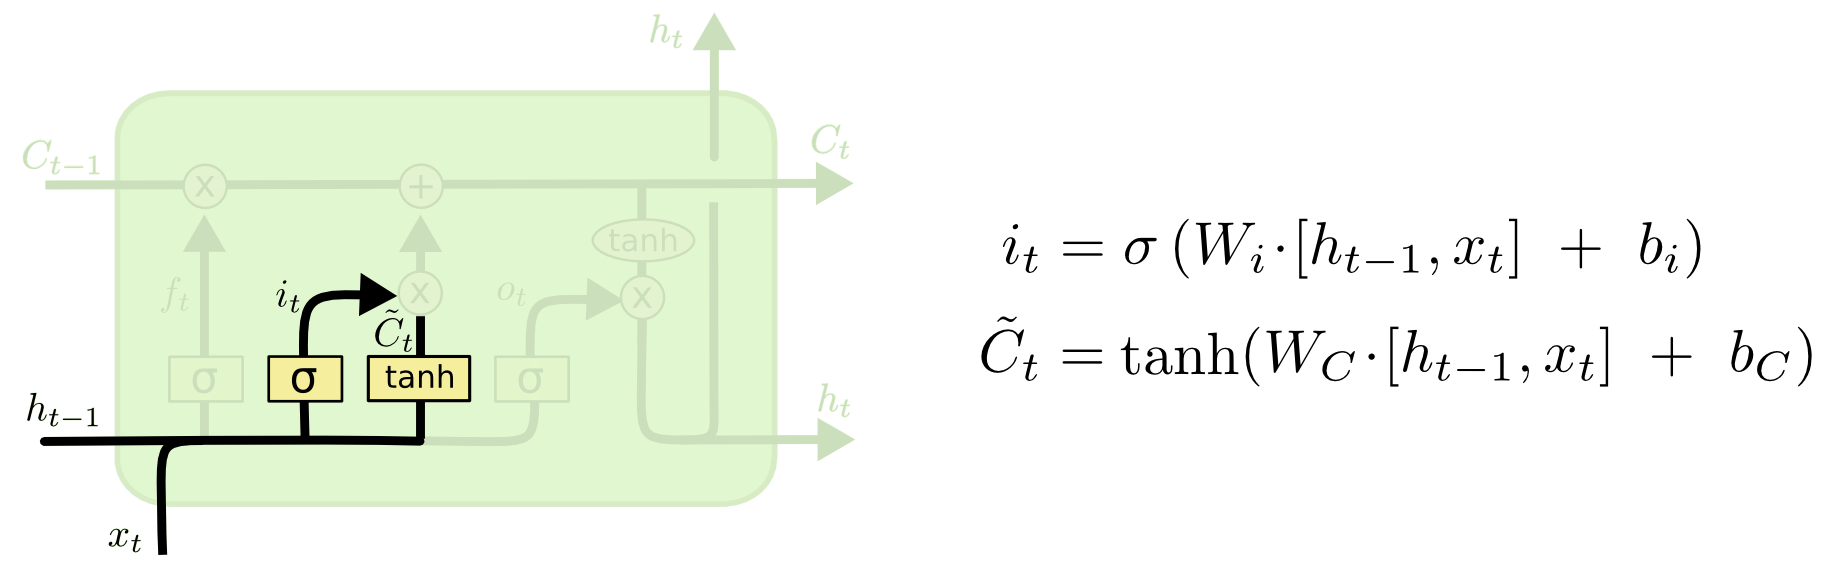
\includegraphics[scale=0.4]{LSTM3-focus-i.png}
    \caption{Ulazna kapija}
    \label{fig:lstm7}
\end{figure}


Sada prethodno stanje ćelije $C_{t-1}$ ažuriramo u novo $C_t$.  Pomnožimo staro stanje sa $f_t$, time zaboravljajući ono što smo odlučili da zaboravimo. Zatim dodamo $i_t \times \tilde{C}_t$. Ovo su potencijalne nove vrednosti, skalirane za onoliko koliko smo odlučili da ažuriramo svaku vrednost stanja (Slika \ref{fig:lstm8}). 

\begin{figure}[htp]
    \centering
    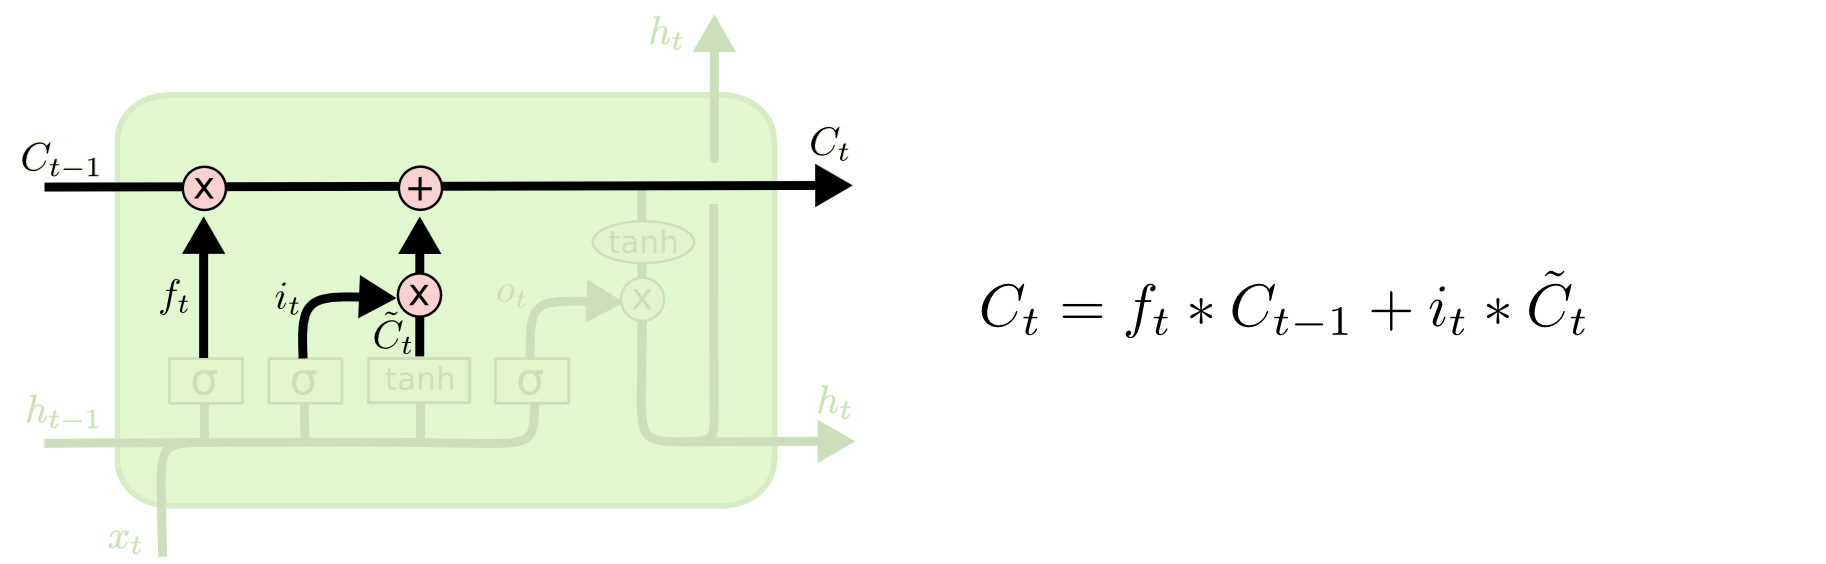
\includegraphics[scale=0.4]{LSTM3-focus-C.png}
    \caption{Računanje novog stanja ćelije}
    \label{fig:lstm8}
\end{figure}


Na kraju je potrebno da odlučimo šta će biti izlaz. Ova vrednost zavisi od stanja ćelije, uz male promene. Prvo prolazimo kroz sloj sa sigmoidnom aktivacionom funkcijom koji odlučuje koje delove ćelije ćemo staviti u izlaz. Zatim prođemo kroz aktivacionu funkciju tangens hiperbolički (kako bismo uokvirili vrednosti u interval između -1 i 1), i pomnožimo sa izlazom iz sloja sa sigmoidnom funkcijom kako bismo u izlaz stavili samo ono što smo odlučili (Slika \ref{fig:lstm9}).

\begin{figure}[htp]
    \centering
    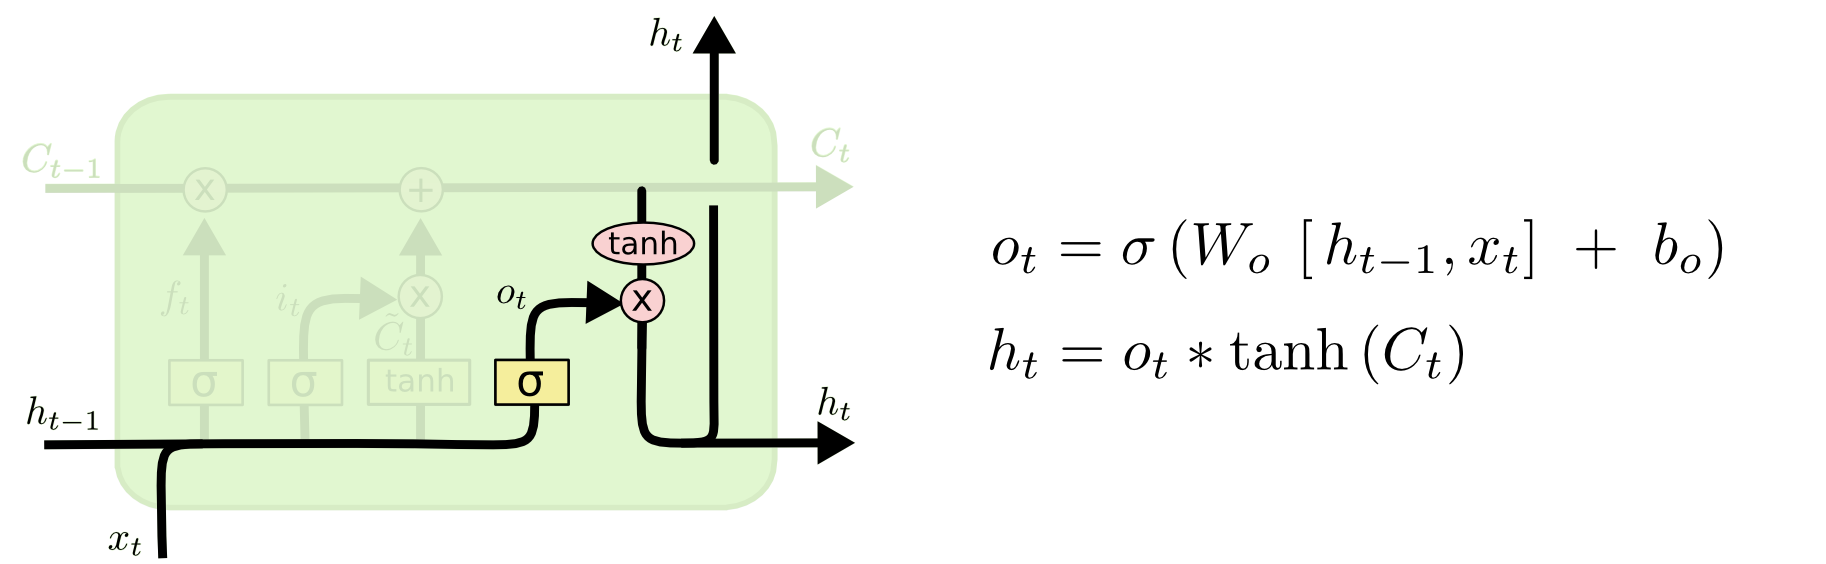
\includegraphics[scale=0.4]{LSTM3-focus-o.png}
    \caption{Računanje izlaza}
    \label{fig:lstm9}
\end{figure}



\section{Problem generisanja teksta}

Generisanje prirodnog jezika (eng. Natural Language Generation - NLG) se intenzivno proučava zahvaljujući bitnim primenama koje ima, kao što su automatsko generisanje dijaloga, automatsko prevođenje jezika, sumarizacija teksta, generisanje opisa fotografija, i mnogih drugih. Poboljšanje kvaliteta automatskog generisanja teksta (u smislu sintakse i semantike) dolazi sa primenom tehnika mašinskog učenja \cite{wang2018automatic}. .

Ovaj rad bavi se automatskim generisanjem teksta na nivou reči. Podaci koje koristimo sadrže kratke opise filmova, preuzete sa vikipedije (mogu se preuzeti sa adrese: \url{https://www.kaggle.com/jrobischon/wikipedia-movie-plots}). Cilj je da se dobije kratak opis neke radnje filma, sa zadatim ulaznim tekstom. Ne očekujemo da rezultati budu precizni, bitno je da predviđeni tekst bude čitljiv.




\section{Zaključak}
\label{sec:zakljucak}




\addcontentsline{toc}{section}{Literatura}
\appendix
\bibliography{bibliografija.bib} 
\bibliographystyle{plain}

\appendix
\section{Dodatak}

\end{document}
